\documentclass[12pt]{article}

\usepackage{report}

\usepackage[utf8]{inputenc} % allow utf-8 input
\usepackage[T1]{fontenc}    % use 8-bit T1 fonts
\usepackage[colorlinks=true, linkcolor=black, citecolor=blue, urlcolor=blue]{hyperref}       % hyperlinks
\usepackage{url}            % simple URL typesetting
\usepackage{booktabs}       % professional-quality tables
\usepackage{amsfonts}       % blackboard math symbols
\usepackage{nicefrac}       % compact symbols for 1/2, etc.
\usepackage{microtype}      % microtypography
\usepackage{lipsum}		% Can be removed after putting your text content
\usepackage{graphicx}
\usepackage{natbib}
\usepackage{doi}
\usepackage{listings}
\usepackage{xcolor}
\usepackage{float}
\usepackage{comment}
\setcitestyle{aysep={,}}




\title{Project Step 2}

\author{List of Group Members\\
\AND\\ 
\AND Brandon Markham
\AND Paul Henson
\AND Sam Arshad
\AND
\AND
\AND
	CS.3339 Computer Architecture\\
\AND
	Texas State University\\
}

% Uncomment to remove the date
\date{March 25, 2024}

% Uncomment to override  the `A preprint' in the header
\renewcommand{\headeright}{Project Step 2 - Turing Machine}
\renewcommand{\undertitle}{The Turing Machine}
\renewcommand{\shorttitle}{}

\definecolor{codegreen}{rgb}{0,0.6,0}
\definecolor{codegray}{rgb}{0.5,0.5,0.5}
\definecolor{codepurple}{rgb}{0.58,0,0.82}
\definecolor{backcolour}{rgb}{0.95,0.95,0.92}

\lstdefinestyle{mystyle}{
    backgroundcolor=\color{backcolour},   
    commentstyle=\color{codegreen},
    keywordstyle=\color{magenta},
    numberstyle=\tiny\color{codegray},
    stringstyle=\color{codepurple},
    basicstyle=\ttfamily\footnotesize,
    breakatwhitespace=false,         
    breaklines=true,                 
    captionpos=b,                    
    keepspaces=true,                 
    numbers=left,                    
    numbersep=5pt,                  
    showspaces=false,                
    showstringspaces=false,
    showtabs=false,                  
    tabsize=2
}

\lstset{style=mystyle}


\begin{document}
\maketitle

\newpage
%\tableofcontents
\thispagestyle{empty}


\newpage
\setcounter{page}{1}
\section{Introduction}
For the second section of the project, the group produced Verilog code to generate arithmetic logic unit (ALU) functions of variable bit widths. Several operations were implemented including bit-wise logic, integer arithmetic, and bit shifting.


\section{Verilog Code}
\label{sec:headings}
In this section, each operation's Verilog code will be shown and explained. Afterward, the code utilized to test the operations will be shown and explained.\\

\textbf{NOTE:} 
Each module includes a parameter \textbf{WIDTH} that determines the number of bits
in the input and output vectors. By specifying different values for \textbf{WIDTH}, these modules may be 
instantiated with different numbers of input/output bits.\\




\subsection{Bit-Wise Logic Modules}
Each multi-bit gate module performs a bit-wise logic operation upon two input vectors `a' and `b' of length \textbf{WIDTH} 
and returns the result of that operation through its output wire `out'.

\subsubsection{Multi-Bit AND Module}
\lstinputlisting[language=Verilog]{Verilog/and_tb.v}

\subsubsection{Multi-Bit NAND Module}
\lstinputlisting[language=Verilog]{Verilog/nand_tb.v}

\subsubsection{Multi-Bit OR Module}
\lstinputlisting[language=Verilog]{Verilog/or_tb.v}

\subsubsection{Multi-Bit NOR Module}
\lstinputlisting[language=Verilog]{Verilog/nor_tb.v}

\subsubsection{Multi-Bit XOR Module}
\lstinputlisting[language=Verilog]{Verilog/xor_tb.v}

\subsubsection{Multi-Bit XNOR Module}
\lstinputlisting[language=Verilog]{Verilog/xnor_tb.v}

\subsubsection{Multi-Bit NOT Module}
\lstinputlisting[language=Verilog]{Verilog/not_tb.v}



\newpage



\subsection{Integer Arithmetic Operations}
\textbf{NOTE:} Operations inside these modules are performed in \textbf{"always"} blocks which 
valuate and update the outputs based on the inputs every time an input changes value. 
The \textbf{"assign"} statements are used to assign the final logic to each output wire. \\

\subsubsection{Binary Multiplier}
The \textbf{binaryMultiplier} module multiplies together two binary numbers provided by inputs \textbf{a} and \textbf{b}. 
The output of this multiplication takes the form of a binary number of twice the length of the original inputs, 
split between its most significant bits and least significant bits across two output wires, \textbf{MSB} and \textbf{LSB}.
\lstinputlisting[language = Verilog]{Verilog/binaryMultiplier.v}

\subsubsection{Binary Adder}
The \textbf{binaryAdder} module performs binary addition. It takes two multi-bit inputs \textbf{a} and \textbf{b} along with a \textbf{carryin} input and produces two outputs: a multi-bit output labelled \textbf{out} \& \textbf{carryout}.
\lstinputlisting[language = Verilog]{Verilog/binaryAdder.v}


\subsubsection{Binary Subtractor}
The \textbf{binarySubtractor}  module performs binary subtraction. It takes two multi-bit inputs \textbf{a} and \textbf{b} along with a \textbf{carryin} input to be used in the case of a borrow bit being necessary when running multiple subtractors in parallel. It produces two outputs: a multi-bit output labelled \textbf{out} \& \textbf{carryout}.
\lstinputlisting[language = Verilog]{Verilog/binarySubtractor.v}

\subsubsection{Binary Divider}
The \textbf{binaryDivision} module performs binary division. It takes two multi-bit inputs \textbf{a} (dividend) \& \textbf{b} (divisor). It produces two outputs, the whole number quotient and the remainder as seen with the output labels \textbf{ans} \& \textbf{rem}.
\lstinputlisting[language = Verilog]{Verilog/binaryDivider.v}

\subsubsection{Bit Shifter}
The \textbf{multiShift} module performs a multi-bit shifting operation. It takes two input \textbf{in} and \textbf{control}.
It produces two multi-bit \textbf{outSubject} (the shifted subject) \& \textbf{outOverflow} (the bits that overflow during shifting).\\
For convenient switching of outputs based on shift direction, 
the outputs of this module are of type `reg' so as to be dynamically assigned inside the \textbf{"always"} block.
\lstinputlisting[language = Verilog]{Verilog/multiShift.v}

\newpage
\subsection{Testbench File}
This testbench code instantiates each type of operation module and applies a number of different input cases to each. This testbench was used to produce the waveforms show later on in this report.\\
While the examples shown in this report use a 4-bit register width, each module was written with scalability in mind. The `BENCHWIDTH' parameter may be scaled to larger sizes in order to produce a ALU operations of higher register sizes.
\lstinputlisting[language=Verilog]{Verilog/Arithmetic_TB.v}

\newpage

\section{Waveform Tests}

In this section we will showcase the wave forms created using our test benches for each circuit we coded in Verilog. We used \textbf{EDAPlayground} and the \textbf{EPWave} generator to create these wave forms. Additionally, the Verilog circuit visualizer at digitaljs.tilk.eu was utilized for efficient testing of modules outside of the context of generating waveforms for this report.\\

\subsection{Bit-Wise Logic Waveforms}
\begin{figure}[H]
    \centering
    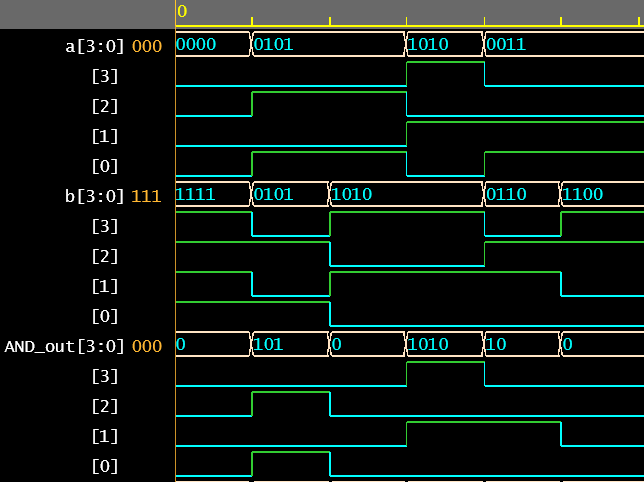
\includegraphics[scale=0.7]{Dr Klepetko/Status 2/figs/AND.PNG}
    \caption{AND Logic Module Waveforms}
    \label{fig:enter-label}
\end{figure}

\begin{figure}[H]
    \centering
    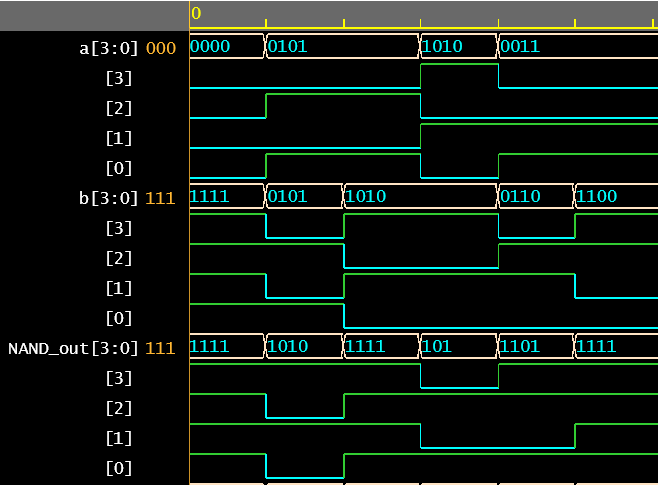
\includegraphics[scale=0.7]{Dr Klepetko/Status 2/figs/NAND.PNG}
    \caption{NAND Logic Module Waveforms}
    \label{fig:enter-label}
\end{figure}

\begin{figure}[H]
    \centering
    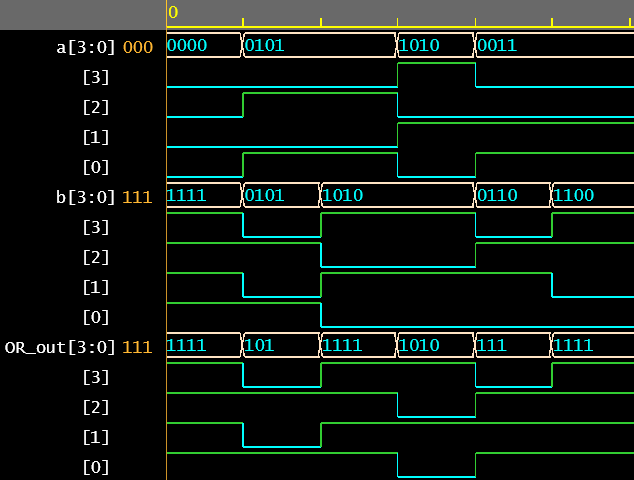
\includegraphics[scale=0.7]{Dr Klepetko/Status 2/figs/OR.PNG}
    \caption{OR Logic Module Waveforms}
    \label{fig:enter-label}
\end{figure}

\begin{figure}[H]
    \centering
    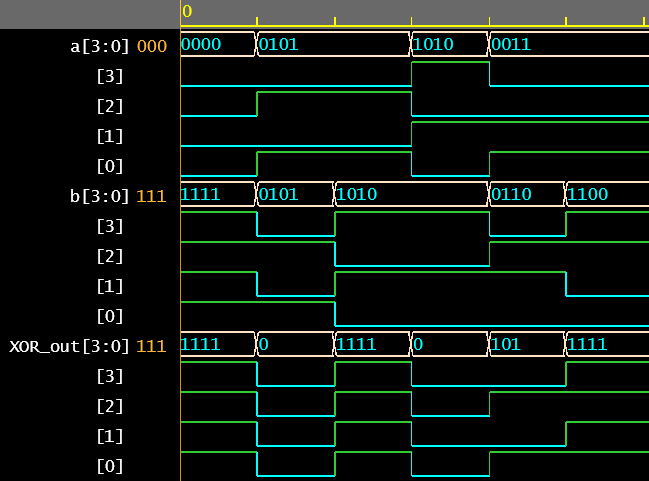
\includegraphics[scale=0.7]{Dr Klepetko/Status 2/figs/XOR.PNG}
    \caption{XOR Logic Module Waveforms}
    \label{fig:enter-label}
\end{figure}

\begin{figure}[H]
    \centering
    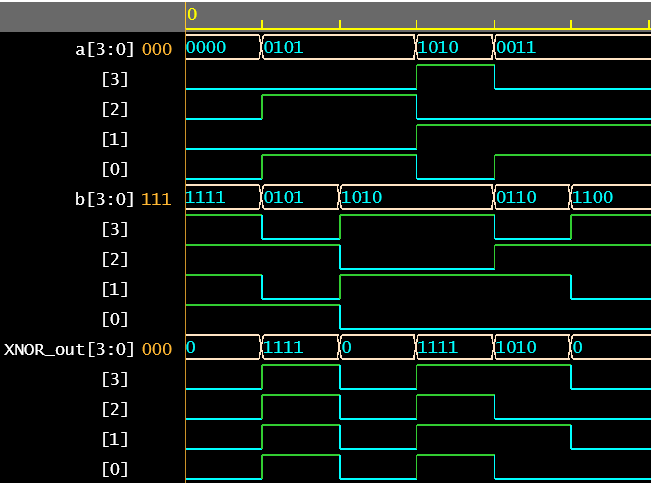
\includegraphics[scale=0.7]{Dr Klepetko/Status 2/figs/XNOR.PNG}
    \caption{XNOR Logic Module Waveforms}
    \label{fig:enter-label}
\end{figure}

\begin{figure}[H]
    \centering
    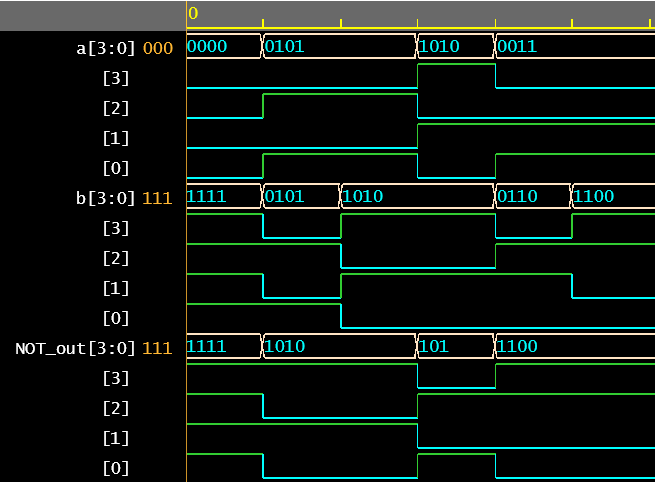
\includegraphics[scale=0.7]{Dr Klepetko/Status 2/figs/NOT.PNG}
    \caption{NOT Logic Module Waveforms}
    \label{fig:enter-label}
\end{figure}


\subsection{Arithmetic Waveforms}
\begin{figure}[H]
    \centering
    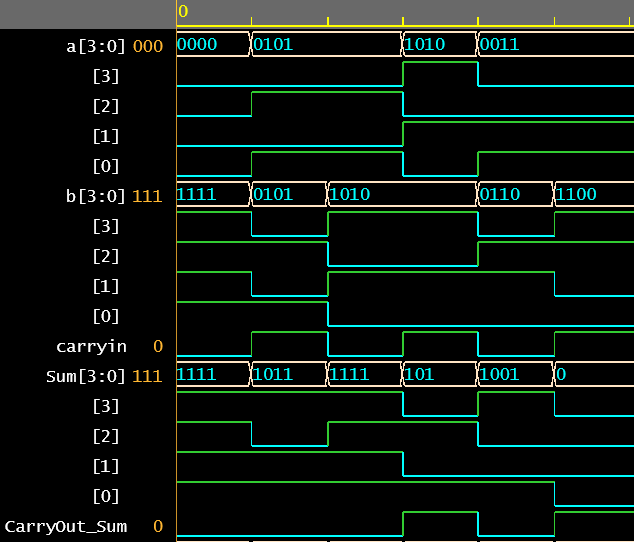
\includegraphics[scale=0.7]{sum}
    \caption{Addition Waveforms}
    \label{fig:enter-label}
\end{figure}

\begin{figure}[H]
    \centering
    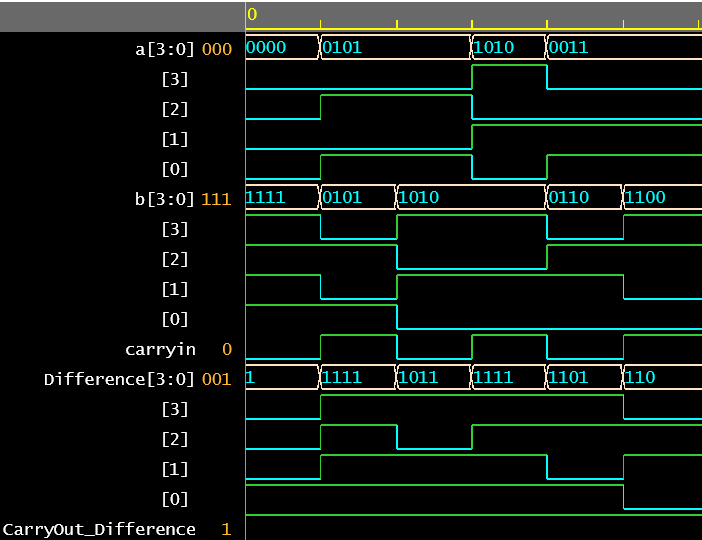
\includegraphics[scale=0.7]{Dr Klepetko/Status 2/figs/difference.PNG}
    \caption{Subtraction Waveforms}
    \label{fig:enter-label}
\end{figure}

\begin{figure}[H]
    \centering
    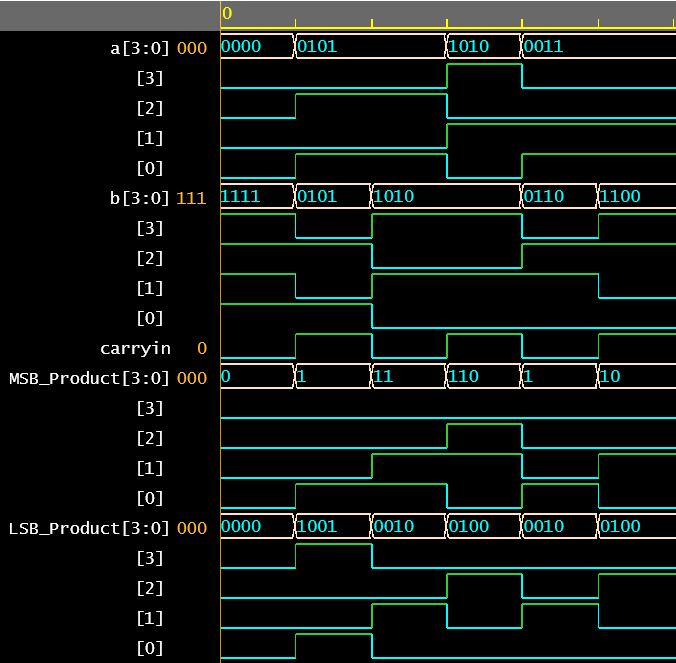
\includegraphics[scale=0.7]{Dr Klepetko/Status 2/figs/product.PNG}
    \caption{Multiplication Waveforms}
    \label{fig:enter-label}
\end{figure}

\begin{figure}[H]
    \centering
    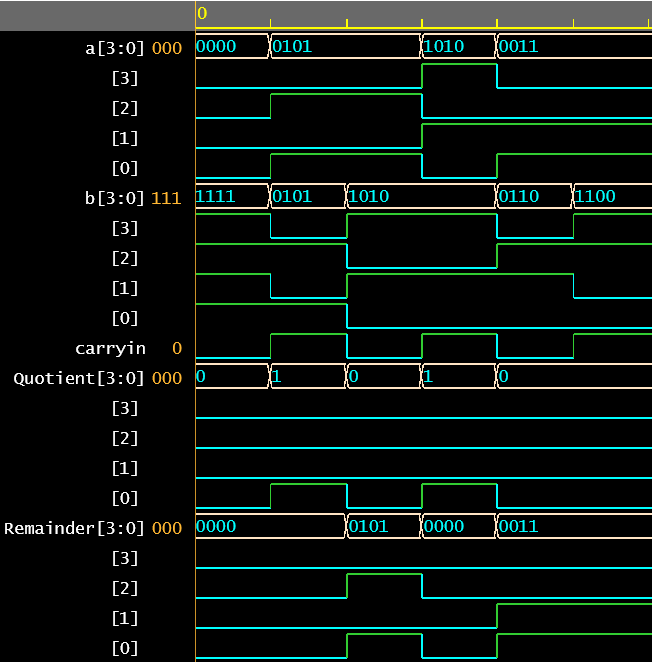
\includegraphics[scale=0.7]{Dr Klepetko/Status 2/figs/divide.PNG}
    \caption{Division Waveforms}
    \label{fig:enter-label}
\end{figure}

\begin{figure}[H]
    \centering
    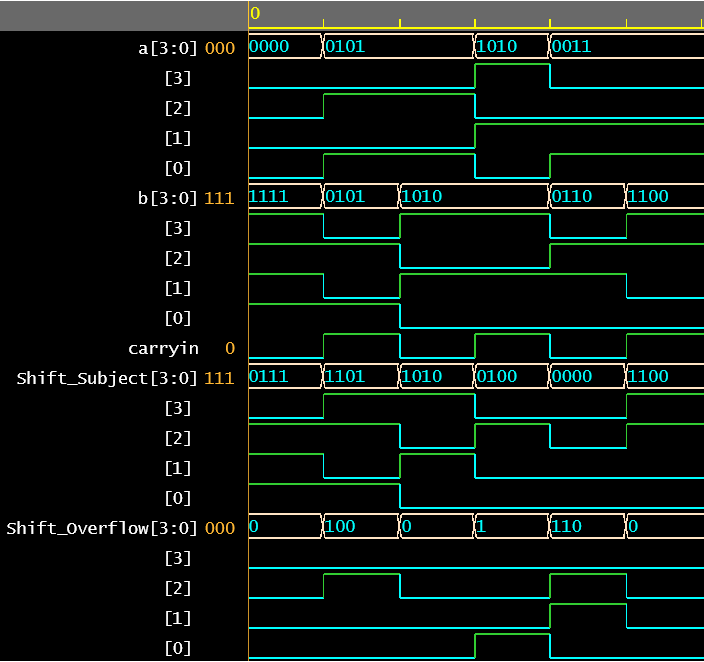
\includegraphics[scale=0.7]{Dr Klepetko/Status 2/figs/shift.PNG}
    \caption{Bitshifting Waveforms}
    \label{fig:enter-label}
\end{figure}

\newpage
\section{Conclusion}

In conclusion, we successfully created and tested the required multi-bit binary logic circuits and arithmetic integer operation modules using using \textbf{EDAPlayground} and its waveform generation feature \textbf{EPWave Waveform Viewer}. Due to misunderstanding instructions, writing the code was challenging until the misunderstanding was clarified. The scale of this project has been greatly simplified in our minds, and we are now nailing down our solutions with the goal of going above and beyond as well as time permits for the final part of the project.

\end{document}



